\chapter{Proposed Approaches}
\label{ch:heuristics}
Heuristics are algorithms to determine a near-optimal solution to a problem. In certain scenarios,
exact methods aren't able to provide the optimal solution in a reasonable amount of time or they can't find it
at all. In contrast, a heuristic is generally capable of offering a solution that is more or less close to
the optimal one.
While there is no assurance regarding the optimality of the provided solution, it may still be considered
acceptable in some instances.
This chapter focuses on explaining the algorithms developed, while the following one presents their evaluation.\\
Before diving into the topic, it is important to understand some of the functions used by all the algorithms.
An action, in order to be eligible for application, must have all its preconditions satisfied in the current state.
If even one precondition is not satisfied, the entire action cannot be applied.
Additionally, applying an action means adding its effects to the current state.
The pseudocode for this function is shown in Algorithm \ref{alg:apply}.

\begin{algorithm}
	\caption{Apply}
	\label{alg:apply}
	\hspace*{0.5em} \textbf{Output}: $newState$
	\begin{algorithmic}[1]
		\Procedure{apply}{$currentState, actionToApply$}
		\State $newState \gets \Call{copy}{currentState}$
		\ForAll{$fact \in actionToApply.effects$}
		\If{$fact \notin newState$}
		\State $newState \gets newState \cup \{fact\}$
		\EndIf
		\EndFor
		\State \textbf{return} $newState$
		\EndProcedure
	\end{algorithmic}
\end{algorithm}

\section{Random}
This is the simplest algorithm implemented, and it is used as a baseline for the evaluation.
At each iteration, it applies a random action from the applicable ones.
It is not a sophisticated or informed solution but this strategy can be useful
in some cases because, by chance, a good plan may be found.
Algorithm \ref{alg:random} shows the pseudocode for it.

\begin{algorithm}
	\caption{Random}
	\label{alg:random}
	\hspace*{0.5em} \textbf{Output}: $solution$
	\begin{algorithmic}[1]
		\Procedure{random}{$planningTask$}
		\State $currentState \gets planningTask.initialState$
		\State $solution \gets [\ ]$ \Comment{Initialize empty solution}
		\While {$planningTask.goalState \not\subseteq currentState$}
		\State $possibleActions \gets \{a \in A \mid pre(a) \subseteq currentState\}$
		\If {$\Call{empty}{possibleActions}$}
		\State \textbf{return} $failure$ \Comment{Infeasible problem}
		\EndIf
		\State $actionToApply \gets \Call{randomChoice}{possibleActions}$
		\State $currentState \gets \Call{apply}{currentState, actionToApply}$
		\State \Call{append}{$solution$, $actionToApply$}
		\EndWhile
		\State \textbf{return} $solution$
		\EndProcedure
	\end{algorithmic}
\end{algorithm}

It is important to notice that if \textit{posissibleActions} is empty, then
a solution to the planning task cannot exist. As said in Chapter \ref{ch:intro},
the problems are Delete-Free|once a fact becomes true in the current state, it remains
true until the end.
Therefore, if there are no actions to apply, it does not mean that the algorithm has reached
a dead end that could be avoided by applying different actions in a different order.
Rather, it indicates that no sequence of actions can lead to the goal state, and therefore no plan exists.
The natural evolution of this approach is to avoid choosing randomly the next action to apply and, instead, use
a strategy to select the action that is more likely to lead to a better plan.

\section{Greedy}
A greedy algorithm is a heuristic that attempts to find an optimal solution by selecting the locally
best possible choice at each iteration. For instance, in our case, the next action to apply will
always be the one with the minimum cost. In the case of a tie, a random action among those with the same cost
will be chosen.
Algorithm \ref{alg:greedy} shows the pseudocode for this algorithm. The omitted parts are identical to those in Algorithm \ref{alg:random}.

\begin{algorithm}
	\caption{Greedy}
	\label{alg:greedy}
	\hspace*{0.5em} \textbf{Output}: $solution$
	\begin{algorithmic}[1]
		\Procedure{greedy}{$planningTask$}
		\State \dots
		\State $possibleActions \gets \{a \in A \mid pre(a) \subseteq currentState\}$
		\If {$\Call{empty}{possibleActions}$}
		\State \textbf{return} $failure$
		\EndIf
		\State $actionToApply \gets \Call{minimumCostAction}{possibleActions}$
		\State \dots
		\EndProcedure
	\end{algorithmic}
\end{algorithm}

Instead of randomly choosing the next action to apply, here the action with minimum cost is always selected.
For this and all subsequent algorithms, if multiple eligible actions share the same minimum (heuristic) cost,
one of them is selected at random.

\section{Revised Max Heuristic}
\label{sec:hmax}
The max heuristic is one of the most well-known delete-relaxation heuristics in the literature.
It is an \textit{admissible} heuristic, meaning that it never overestimates the cost of reaching the goal.
It assigns an heuristic cost to each action based on Equation \ref{eq:hmax} and \ref{eq:cost}

\begin{equation}
	\label{eq:hmax}
	h_{max}\left(p;s\right) \coloneqq \begin{cases}
		0                                                                & \text{if $p \in s$} \\
		\text{min}_{a \in O\left(p\right)}\left[h\left(a;s\right)\right] & \text{otherwise}
	\end{cases}
\end{equation}

where $h_{max}\left(p;s\right)$ stands for an estimate of the cost of achieving the fact \textit{p} from
the current state \textit{s}, $O\left(p\right)$ is the set of actions $\{a \in A \mid p \in \textit{eff(a)}\}$, and

\begin{equation}
	\label{eq:cost}
	h\left(a;s\right) \coloneqq cost(a) + \text{max}_{q \in pre\left(a\right)} \left[h(q, s)\right]
\end{equation}

stands for the cost of achieving the preconditions of an action \textit{a} and applying it.\\
The idea behind the use of this heuristic is similar to that of the greedy approach.
While in the greedy approach the action with the minimum actual cost is chosen, in this case,
the action with the minimum heuristic cost is selected at each iteration.
This thesis presents an implementation of the max heuristic that goes a step further.
By definition, any action applicable in the current state has a heuristic cost equal to
its own cost, since all its preconditions are satisfied|regardless of whether the action is
actually useful for reaching the goal state or not.
The implemented version performs a technique called \textit{pruning}, which consists of assigning
an infinite cost to useless actions|indicating that these actions are not helpful in finding a good plan.
As a result, such actions are effectively excluded from consideration when selecting the next action to apply,
while the remaining ones retain their correct heuristic cost.
The pseudocode for this algorithm is presented in Algorithm \ref{alg:hmax} and \ref{alg:greedyhmax}.

\begin{algorithm}
	\caption{Max Heuristic}
	\label{alg:hmax}
	\hspace*{0.5em} \textbf{Output}: $minHcost$
	\begin{algorithmic}[1]
		\Procedure{hmax}{$currentState, fact$}
		\If {$fact \in currentState$}
		\State \textbf{return} 0 \Comment{Base case}
		\EndIf
		\State $actions \gets \{a \in A \mid fact \in \textit{eff(a)}\}$ \Comment{Get all the actions having \textit{fact} as effect}
		\If {$\Call{empty}{actions}$}
		\State \textbf{return} $+\infty$ \Comment{The fact is unreachable}
		\EndIf
		\State $minHcost \gets +\infty$
		\ForAll{$action\in actions$}
		\State $maxCost \gets 0$
		\ForAll {$pre \in action.preconditions$}
		\State $maxCost \gets \Call{max}{maxCost, \Call{hmax}{currentState, pre}}$
		\EndFor
		\State $action.hCost \gets action.cost + maxCost$
		\State $minHcost \gets \Call{min}{minHcost, action.hCost}$
		\EndFor
		\State \textbf{return} $minHcost$
		\EndProcedure
	\end{algorithmic}
\end{algorithm}

\begin{algorithm}
	\caption{Greedy Search with Max Heuristic}
	\label{alg:greedyhmax}
	\hspace*{0.5em} \textbf{Output}: $solution$
	\begin{algorithmic}[1]
		\Procedure{greedyHmax}{$planningTask$}
		\State \dots
		\ForAll {$a \in A$}
		\State $a.hCost \gets \infty$ \Comment{Initialize actions' heuristic cost}
		\EndFor
		\State $estimatedCost \gets 0$
		\ForAll {$goal \in planningTask.goalState$}
		\State $estimatedCost \gets \Call{max}{estimatedCost, \Call{hmax}{currentState, goal}}$
		\EndFor
		\State $possibleActions \gets \{a \in A \mid pre(a) \subseteq currentState\}$
		\If {$\Call{empty}{possibleActions}$}
		\State \textbf{return} $failure$
		\EndIf
		\State $actionToApply \gets \Call{minimumHcostAction}{possibleActions}$
		\State \dots
		\EndProcedure
	\end{algorithmic}
\end{algorithm}

Starting from each fact in the goal state, \verb|HMAX| is called to perform a backward cost propagation.
In this way, all useless actions are implicitly ignored and retain their original cost,
which remains set to $+\infty$.
When selecting the next action to apply, any action with an infinite cost will be ignored,
and the one with the lowest heuristic cost among the remaining options will be chosen.
Figures \ref{fig:hmax_scheme} and \ref{fig:hmax_pruning_scheme} can help visualize the concept.

\begin{figure}[htbp]
	\centering
	\begin{minipage}{0.45\textwidth}
		\centering
		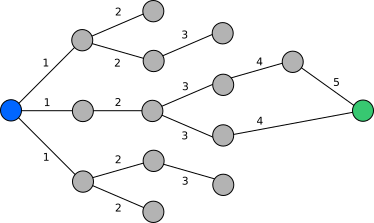
\includegraphics[width=\linewidth]{images/hmax.png}
		\caption{Caption for left figure}
		\label{fig:hmax_scheme}
	\end{minipage}
	\hspace{0.05\textwidth}
	\begin{minipage}{0.45\textwidth}
		\centering
		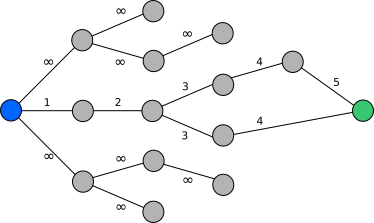
\includegraphics[width=\linewidth]{images/hmax_pruning.png}
		\caption{Caption for right figure}
		\label{fig:hmax_pruning_scheme}
	\end{minipage}
\end{figure}

As previously mentioned, any action that can be applied from
the current state will always have a heuristic cost equal to its actual cost.
Therefore, this algorithm can be seen as a greedy + pruning approach: it selects the next action based on the action's cost,
while discarding useless actions.
To observe the true behavior of the proposed algorithm, it should ideally be used within the context of the \verb|A*| algorithm,
a well-known search strategy that combines actual cost from the start with a heuristic estimate to the goal.
Specifically, \verb|A*| selects actions by minimizing the function $f(n) = g(n) + h(n)$, where $g(n)$ is the cost
required to reach node $n$, and $h(n)$ is the estimated cost to reach the goal state from $n$.
\verb|A*| selects actions based on the sum of these two values, leading to optimal solutions when an admissible heuristic, such as \verb|HMAX|, is used.
However, since \verb|A*| was not implemented in this thesis, an alternative approach was used to evaluate the algorithm's actual performance.

\section{Max Heuristic + Lookahead}
As mentioned in the previous section, the presented algorithm can be considered a greedy + pruning approach,
since the full potential of the heuristic cannot be exploited|the heuristic cost of the applicable actions is always equal
to the actions' actual cost.
To evaluate its performance, a new version of the heuristic is proposed.
Instead of selecting the action with the minimum cost, the algorithm tries each possible action,
recomputes the \verb|HMAX| value for each resulting state, and finally applies the action that leads to the state with the lowest
new heuristic value.
The pseudocode for this approach is shown in Algorithm \ref{alg:lookahead} and \ref{alg:hmaxlookahead}.

\begin{algorithm}
	\caption{Lookahead}
	\label{alg:lookahead}
	\hspace*{0.5em} \textbf{Output}: $actionToApply$
	\begin{algorithmic}[1]
		\Procedure{lookahead}{$currentState, possibleActions$}
		\ForAll{$action\in possibleActions$}
		\State $newState \gets \Call{apply}{currentState, action}$
		\State $estimatedCost \gets 0$
		\ForAll {$goal \in planningTask.goalState$}
		\State $estimatedCost \gets \Call{max}{estimatedCost, \Call{hmax}{newState, goal}}$
		\EndFor
		\State $action.hCost \gets action.hCost + estimatedCost$
		\EndFor
		\State $actionToApply \gets \Call{minimumHcostAction}{possibleActions}$
		\State \textbf{return} $actionToApply$
		\EndProcedure
	\end{algorithmic}
\end{algorithm}

\begin{algorithm}
	\caption{Max Heuristic with Lookahead}
	\label{alg:hmaxlookahead}
	\hspace*{0.5em} \textbf{Output}: $solution$
	\begin{algorithmic}[1]
		\Procedure{hmaxLookahead}{$planningTask$}
		\State \dots
		\State $estimatedCost \gets 0$
		\ForAll {$goal \in planningTask.goalState$}
		\State $estimatedCost \gets \Call{max}{estimatedCost, \Call{hmax}{currentState, goal}}$
		\EndFor
		\State $possibleActions \gets \{a \in A \mid pre(a) \subseteq currentState\}$
		\If {$\Call{empty}{possibleActions}$}
		\State \textbf{return} $failure$
		\EndIf
		\State $actionToApply \gets \Call{lookahead}{currentState, possibleActions}$
		\State \dots
		\EndProcedure
	\end{algorithmic}
\end{algorithm}

The algorithm "looks ahead" at the heuristic cost of the state resulting from each possible action,
and then applies only the action that appears to be the most convenient.

\section{Novel Heuristic}
\label{sec:shortestpath}
In this section, a completely new approach is introduced. As discussed in Section \ref{sec:hmax},
the modified version of the max heuristic ultimately behaves like a greedy + pruning algorithm, limiting its effectiveness.
Here, we aim to use the same backward propagation mechanism, but with a different heuristic cost assigned to each action.
The core idea is to assign each action a cost that estimates its actual distance to the goal.
Specifically, the cost assigned to an action corresponds to the cost of the \textit{shortest path} to reach a fact in the goal state.
The mathematical formalism is presented in Equations \ref{eq:sp} and \ref{eq:spcost}:

\begin{equation}
	\label{eq:sp}
	h_{sp}\left(p;s_*\right) \coloneqq \begin{cases}
		0                                                                    & \text{if $p \in s_*$} \\
		\text{min}_{a \in O\left(p\right)}\left[h_a\left(a;s_*\right)\right] & \text{otherwise}
	\end{cases}
\end{equation}

Here, $h_{sp}\left(p;s_*\right)$ denotes the estimated cost of achieving a fact in the goal state $s_*$, starting from
fact \textit{p}. The set $O\left(p\right)$ represents the actions that produce \textit{p} as an effect,
that is, $O\left(p\right) = \{a \in A \mid p \in \textit{eff(a)}\}$. The function $h_a\left(a;s_*\right)$ is
defined as follows:

\begin{equation}
	\label{eq:spcost}
	h_a\left(a;s_*\right) \coloneqq cost(a) + \text{min}_{q \in \textit{eff}\left(a\right)} \left[h_{sp}\left(q;s_*\right)\right]
\end{equation}

This espression estimates the cost of achieving a fact in the goal state $s_*$ by applying
action \textit{a}. The heuristic cost of an action is defined as its own cost plus the minimum estimated cost among its effects.
In this way, each action is assigned a heuristic cost corresponding to the cost of the shortest path to reach
a fact in the goal state.
The actual implementation of this algorithm uses a \textit{priority queue} to ensure an
efficient and iterative computation. The pseudocode is presented in Algorithm \ref{alg:sp}.

\begin{algorithm}
	\caption{Shortest Path Heuristic}
	\label{alg:sp}
	\hspace*{0.5em} \textbf{Output}:
	\begin{algorithmic}[1]
		\Procedure{shortestPath}{$currentState, goalState$}
		\State $factCosts \gets \{+\infty, \dots, +\infty\}$ \Comment{Initialize facts' cost to $+\infty$}
		\State $pq\gets \{\}$ \Comment{Empty priority queue}
		\ForAll {$goal \in goalState$}
		\State $factCosts[goal] \gets 0$
		\State $\Call{push}{pq, goal, 0}$
		\EndFor
		\While {$!\Call{empty}{pq}$}
		\State $fact \gets \Call{pop}{pq}$ \Comment{Get the fact having minimum cost}
		\If {$fact \in currentState$}
		\State \textbf{continue} \Comment{Do not propagate the cost}
		\EndIf
		\State $actions \gets \{a \in A \mid fact \in \textit{eff}\left(a\right)\}$
		\ForAll {$action \in actions$}
		\State $newCost \gets action.cost + factCosts[fact]$
		\If {$newCost >= action.hCost$}
		\State \textbf{continue}
		\EndIf
		\State $action.hCost = newCost$
		\ForAll {$pre \in action.preconditions$}
		\If {$newCost < factCosts[pre]$}
		\State $factCosts[pre] \gets newCost$
		\If {$\Call{has}{pq, pre}$}
		\State $\Call{change}{pq, pre, newCost}$
		\Else
		\State $\Call{push}{pq, pre, newCost}$
		\EndIf
		\EndIf
		\EndFor
		\EndFor
		\EndWhile
		\EndProcedure
	\end{algorithmic}
\end{algorithm}

The priority queue internally maintains the facts ordered by increasing cost.
Each time a fact is removed from the queue, it is the one with the minimum heuristic cost.
The heuristic cost of each action having the removed fact as an effect is then updated accordingly,
and all of its preconditions are subsequently inserted into the queue.
In this way, all useful actions will be assigned a cost equal to the shortest path to reach a fact in
the goal state, while useless actions will retain an infinite cost.
The usage of this algorithm is analogous to what was presented in Algorithm \ref{alg:greedyhmax}.
